\documentclass{sig-alternate}

\usepackage[usenames, dvipsnames]{color}
\usepackage{times}
\usepackage{xspace}
\usepackage{textcomp}
\usepackage{wrapfig}
\usepackage{graphicx}
\usepackage{url}
\usepackage{amsmath, amssymb}
\usepackage[protrusion=true,expansion=true]{microtype}
\usepackage{comment}
\usepackage{alltt}
\usepackage{appendix}
%\usepackage{algorithm}
%\usepackage{algorithmic}
\usepackage{booktabs}
\usepackage{color}
\usepackage{listings}
\lstset{ %
basicstyle=\ttfamily\scriptsize,       % the size of the fonts that are used for the code
numbers=left,                   % where to put the line-numbers
numberstyle=\ttfamily,      % the size of the fonts that are used for the line-numbers
%aboveskip=0pt,
%belowskip=0pt,
stepnumber=1,                   % the step between two line-numbers. If it is 1 each line will be numbered
%numbersep=10pt,                  % how far the line-numbers are from the code
breakindent=0pt,
firstnumber=0,
%backgroundcolor=\color{white},  % choose the background color. You must add \usepackage{color}
showspaces=false,               % show spaces adding particular underscores
showstringspaces=false,         % underline spaces within strings
showtabs=false,                 % show tabs within strings adding particular underscores
frame=leftline,
tabsize=2,  		% sets default tabsize to 2 spaces
captionpos=b,   		% sets the caption-position to bottom
breaklines=false,    	% sets automatic line breaking
breakatwhitespace=true,    % sets if automatic breaks should only happen at whitespace
%escapeinside={\%}{)}          % if you want to add a comment within your code
columns=fullflexible,
% are you fucking kidding me lstlistings?  who puts the line numbers outside the margin?
xleftmargin=6mm,
xrightmargin=-6mm,
numberblanklines=false,
language=Ruby,
morekeywords={declare,table,scratch,channel,interface,include}
}
\lstset{escapeinside={(*}{*)}}
%\renewcommand*\thelstnumber{\the\value{lstnumber}:}


%\linespread{0.975}

\usepackage{txfonts}

% \newcommand{\jmh}[1]{{\textcolor{red}{#1 -- jmh}}}
 \newcommand{\paa}[1]{{\textcolor{blue}{#1 -- paa}}}
% \newcommand{\rcs}[1]{{\textcolor{green}{#1 -- rcs}}}
% \newcommand{\nrc}[1]{{\textcolor{magenta}{#1 -- nrc}}}
% \newcommand{\wrm}[1]{{\color{BurntOrange}{#1 -- wrm}}}
% \newcommand{\kc}[1]{{\textcolor{cyan}{#1 -- kc}}}
\newcommand{\smallurl}[1]{{\small \url{#1}}}

\CopyrightYear{2011}
\conferenceinfo{CIDR}{'11 Asilomar, California USA}

\begin{document}
\title{Consistency Analysis in Bloom: a CALM and Collected Approach}

\numberofauthors{4}
\author{
Peter Alvaro, Neil Conway, Joseph M. Hellerstein, William R. Marczak \vspace{12pt} \\
\{palvaro, nrc, hellerstein, wrm\}@cs.berkeley.edu \\
University of California, Berkeley
}

\maketitle

\begin{abstract}
  Distributed programming has become a topic of widespread interest, and many
  programmers now wrestle with tradeoffs between data consistency, availability
  and latency.  Distributed transactions are often rejected as an undesirable
  tradeoff today, but in the absence of transactions there are few concrete
  principles or tools to help programmers design and verify the correctness of
  their applications.

  We address this situation with the \emph{CALM} principle, which connects the
  idea of distributed consistency to program tests for logical monotonicity.  We
  then introduce \emph{Bloom}, a distributed programming language that is
  amenable to high-level consistency analysis and encourages order-insensitive
  programming.  We present a prototype implementation of Bloom as a
  domain-specific language in Ruby. We also propose a static analysis technique
  that identifies {\em points of order} in Bloom programs: code locations where
  programmers need to inject coordination logic to ensure consistency.  We
  illustrate these ideas in the context of two variants of a distributed
  ``shopping cart'' application in Bloom.  We also sketch the feasibility of
  code rewrites to support runtime annotation of data consistency, a topic for a
  longer paper.
\end{abstract}

\section{Introduction} 
\label{sec:intro} 
Although distributed programming has become an essential and commonplace task,
it remains very challenging for most developers to write correct distributed
programs. The inherent difficulties of distributed computing---concurrency,
asynchrony, and partial failure---are exacerbated by the scale at which modern
distributed systems operate.

% remind reviewers that it's a database problem. can remove if accepted! 
Much of the discussion about distributed programming today revolves around data
management systems, and the tradeoffs between transactions and loose
consistency. Programmers using distributed transactions are relieved of
consistency concerns but often face significant performance and operational
challenges~\cite{Birman2009}. By contrast, programmers who use loosely
consistent systems can expect more predictable and low-latency performance, but
must reason explicitly about program correctness over inconsistent distributed
state.

In recent years there has been increased interest in techniques to help
programmers achieve correct program behavior without requiring strongly
consistent storage. This idea has been explored in two different frameworks,
\emph{Convergent Objects} and \emph{Monotonic Logic}.

\vspace{0.5em}\noindent
\textbf{Convergent Objects}: In this approach, a programmer writes encapsulated
object classes whose public methods guarantee certain properties regarding
message reordering and/or retry. For example, Statebox is an open-source library
that merges conflicting updates to data items in a key-value store; the user of
the library need only register commutative, idempotent merge
functions~\cite{statebox}. This approach has roots in research in
databases~\cite{Farrag1989,Garcia-Molina1983,Helland2009} and
groupware~\cite{Ellis1989,Sun1998}.  Shapiro et al.\ recently proposed a model
for these approaches called \emph{Conflict-Free Replicated Data Types} (CRDTs),
which formalizes these ideas in an algebraic framework~\cite{Shapiro2011b}.

The main problem with the CRDT approach is that its guarantees of correctness
are limited to an individual replicated data value, not to application logic in
general. For example, consider a distributed algorithmic trading service that
uses a CRDT to represent a mutable set \texttt{Portfolio}. Suppose one server
$M$ reads a local version of the set containing an element \texttt{BNNA} and
constructs an expected portfolio value $v = f(\mbox{\texttt{Portfolio}})$
derived from that version. Concurrently, \texttt{BNNA} is removed from the local
version of \texttt{Portfolio} at another server $N$. The CRDT can ensure that
$M$ and $N$ will eventually agree that \texttt{BNNA} is absent from the set, but
the application state at $M$ and $N$ may remain inconsistent unless the value
$v$ at $M$ is updated to reflect the removal of \texttt{BNNA}. Although the CRDT
maintains its own invariants, the programmer still bears the burden of ensuring
the consistency semantics of the entire program.

\vspace{0.5em} \noindent
\textbf{Monotonic Logic}: In recent work, we observed that the database theory
literature on non-monotonic logic provides a promising starting point for
reasoning about distributed consistency. Intuitively, a \emph{monotonic} program
computes more information over time---it never ``retracts'' an earlier
conclusion in the face of new information. We proposed the CALM
theorem~\cite{Hellerstein2010}, which established that all monotonic programs
are eventually consistent~\cite{Ameloot2011,dedalus-pods12-tr}. Monotonicity of
a Datalog-style program is straightforward to determine conservatively from
syntax, so the CALM theorem provides the basis for a simple analysis technique
for verifying the consistency of distributed programs~\cite{Alvaro2011}. We
realized the CALM analysis as part of Bloom, a Datalog-based DSL for distributed
programming~\cite{bloom}.

The original formulation of Bloom and CALM only validated consistency for programs that compute sets of facts that grow over time (``set monotonicity''); that is, ``growth'' is defined according to set containment. As a practical matter, this is overly conservative: several common distributed programming idioms that are monotonic do not satisfy syntactic monotonicity tests for Datalog. In particular, threshold tests over monotonic aggregate values (e.g., ``$\mathrm{max}(S) > k$'') and upward-moving mutable counters are both considered to be non-monotonic by the original CALM analysis.  As a result, the initial Bloom prototype advises the programmer to guard those constructs with strong consistency methods like Paxos~\cite{Lamport1998} or Two-Phase Commit. 

\subsection{A Hybrid Approach}
% The strengths and weaknesses of these two approaches appear complementary. CRDTs provide synchronization-free consistent objects, but cannot guarantee whole-program consistency. Bloom's CALM analysis guarantees whole-program consistency but is unable to verify a number of natural coordination-free mechanisms.
In this paper, we extend our previous work to accommodate the ideas underlying CRDTs. Instead of only allowing growth according to the set containment
partial order, we allow any user-defined partial order to be used.  
We do this by providing \emph{join semi-lattices} as a programming construct.
We give a
formal definition of this construct below, but the intuition is that the programmer provides a commutative, idempotent merge function (``least upper bound'')
that takes two input values and produces an output value that is not smaller
than either of the input values (according to the user's partial order). This
generalizes Bloom (and traditional Datalog), which assumes a fixed merge
function (set union) and partial order (set containment).
% Relate user-defined merge functions to merge functions in other contexts?
% (e.g., key-value store, COPS, Piccolo)

% Explain how lattices generalize monotonic datalog
It is attractive to incorporate join semi-lattices into logic programming,  but doing so raises challenges in language design, consistency analysis and efficient execution.  In this paper, we make the following contributions:
\begin{enumerate}
% \item
%   We present \baselang, a variant of Datalog that is defined over lattices. We
%   define a model-theoretic semantics for \baselang, and show that \baselang
%   generalizes Datalog.

\item
  We introduce \lang, an extension of Bloom that supports lattices. We detail
  the builtin lattice types provided by \lang and show how developers can
  define new lattices.
  
\item 
  We provide interfaces for consistency-preserving mappings across lattices via
  \emph{morphisms} and \emph{monotonic functions}.  This is critical for \lang
  and forms a useful extension to the CRDT framework as well.

\item 
  We generalize the CALM analysis to programs that contain both lattices and
  set-oriented collections, and show how lattices can be used to prove the
  confluence of several common distributed design patterns that were regarded as
  non-monotonic in Bloom. % XXX: revisit this

\item
  For efficient execution, we show how to extend the standard Datalog semi-naive
  evaluation scheme~\cite{Balbin1987} to support both lattices and traditional
  database relations. We also describe how an existing Datalog engine can be
  extended to support lattices with relatively minor changes.

\item
  Finally, we demonstrate the usefulness of lattices with two case studies.
  First we revisit the simple e-commerce scenario presented in Alvaro et al., in
  which clients interact with a replicated shopping cart
  service~\cite{Alvaro2011}. We show how \lang can be used to make the
  ``checkout'' operation monotonic, despite the fact that it requires
  aggregating over a distributed data set.

  Second, we use \lang to implement vector clocks and causal delivery, two
  standard building blocks for distributed programming. We show how both
  algorithms can be realized as monotonic \lang programs that are concise and
  readable.
\end{enumerate}

\section{Consistency and Monotonicity}

The principal issue in maintaining consistency in distributed systems is {\em
temporal nondeterminism} -- the delay and re-ordering of data exchanged between
nodes.  A sufficient condition for consistency in a distributed system is {\em
order independence} -- the independence of the execution from temporal
nondeterminism.

\wrm{a bit out of my depth here talking about database operators}

Thinking about a query plan for a relational language, such as SQL or Datalog,
we see that there are two types of operators.  A {\em monotonic} operator, such
as a join, selection, or projection, can produce part of the final output
immediately if the input tuples satisfy a certain condition.  In the case of a
join, if the input tuples arrive on-line (i.e. over the network), we must
materialize them in order to compute the full join.  A non-monotonic operator,
such as an antijoin or aggregate, cannot produce any final output until it
views some nontrivial subset of the input tuples -- possibly the entire set.

The key difference between distributing monotonic and non-monotonic operators
is that a non-monotonic operator cannot produce output until it is sure it has
seen the entire set of tuples it needs to see.  If a non-monotonic operator is
allowed to prematurely produce output, it may report an incorrect result.  For
example, a sum aggregate over a set may produce an incorrect result if only a
subset of the tuples are summed, and an antijoin may output an incorrect row if
it does not examine all the input tuples.

If correctness is desired, non-monotonic operators must have {\em coordination
logic} -- code that transmits auxilliary information about set completeness,
that the non-monotonic operator uses to produce a correct result.  The
non-monotonic operator orders the production of the result only after it has
examined the complete set.  Our language, {\em Bud}, omits coordination logic
from non-monotonic operators by default, and forces the user to specify it.
This is because badly-designed coordination logic can be a performance penalty,
and this seems like a hard problem for an optimizer to approximate (an exact
solution is undecidable).  In any case, this is the hard component of
distributed systems programming, so a language should focus programmer effort
on it.  Monotonic operators require no coordination logic.

A simple conservative check for monotonicity of a program is syntactic -- if a
program contains any symbols that are known to correspond to non-monotonic
operators (such as "NOT", and certain aggregate symbols "MIN >", "MAX <"), then
it is non-monotonic, otherwise it is monotonic.  Note it is interesting that
"MIN <" and "MAX >" are monotonic \wrm{and this somehow corresponds to escrow
transactions, though i don't see the connection...}  A more advanced
whole-program static analysis would take into account whether any non-monotonic
symbols correspond to portions of the query plan that are ever used
(satisfiable) -- also undecidable, but conservative tests with constraint
propagation are possible.  It may also be useful to understand which portions
of the program's execution or output may be affected by network
non-determinism, and which are deterministic.  In this case, a static or
runtime analysis could perform {\em taint tracking} of network nondeterminism.
%Intuitively, a tuple is tainted if it is the transitive result of some
%non-monotonic operator.

This monotonicity analysis can also be used to identify the non-monotonic
pieces in the program.  The output of this analysis is an overestimate of the
loci in the program that require coordination in order to ensure consistency.
We call the loci suggested by this analysis the program's {\em points of
order}.  The user can augment the program with appropriate coordination logic.
In the general case, it is undecidable to verify whether they have done this
correctly.  In fact, the introduction of coordination logic may involve
additional non-monotonic operators (for example, two-phase commit has a
non-monotonic "COUNT users = COUNT messages" statement).  There are a variety
of possible solutions to this problem.  One option is for expert programmers
(i.e. us) to encapsulate a suite of coordination protocols in a library, and
manually verify the correctness of each protocol.  Another option is to develop
various static analyses in the style of stratification tests for Datalog.
\wrm{not sure how we can introduce additional detail here without pulling in
tons of knowledge dependencies} 

\wrm{addressed this} \jmh{At minimum, we should assert formal proof in one
direction: purely Monotonic deduction can be done without coordination.  Start
with explaining syntactic montonicity, perhaps via SQL, Datalog and MapReduce.
Then enrich this by saying that single-node non-monotonicity is OK (if it's
acyclic).} \wrm{i don't think it's okay if it's acyclic -- it's only okay if it
does not depend on any network messages}  \jmh{  We should then enrich further
by introducing the non-syntactic, ``instance-oriented'''' style monotonicity:
saying that individual monotonic deductions---i.e. any monotonic tuple
lineage---can be computed without coordination.  Give intuitive examples that
are database instance-dependent (a la local stratification), and that are
program-semantics dependent (a la universal constraint stratification).  The
latter should do escrow transactions, and/or tee up shopping cart.}

\wrm{addressed this} \jmh{Now you can talk at least in casual terms about a
check for consistency: check the program for non-monotonicity.  Can probably do
intuition of the data dependency here, and hint at how we'll do taint tracking
later.}

\wrm{not sure if this is true, also not sure what "universal-constraint-style
analyses" you are referring to} \jmh{Now that we've said that ``counting
requires waiting'', point out that ``waiting requires counting'': coordination
protocols are basically threshhold tests on distributed count aggregates.
Hence any check for consistency like the one above will flag the coordination
logic as a problem.  Our solution: either expert programmers (us) verify the
modules, or we develop universal-constraint-style analyses to validate them.}

\wrm{i think we decided the other direction of CALM was false.  consider
committed choice.  that's non-monotonic any way you look at it (except for the
definition I tried to sell you durig the POPL submission that we ultimately
rejected, because we believed monotonic should mean "has a monotonic
representation in FOL")} \jmh{Finally, introduce the Bi-directional CALM
Conjecture: that non-monotonic deduction (at the individual tuple level)
requires coordination.  We can wave hands here about this requiring a crisper
definition of coordination than we needed before.}

\wrm{not sure what this means} \jmh{Occurs to me there's a disconnect here with
the intro---in the intro we said that programming without coordination relates
to ``loose'' consistency.  We should show a case where for the
universal-constraint scenario, a read-write consistency analysis would flag
this as bad, and a transaction manager would forbid it.}

\section{Adding Lattices to Bloom}
\label{sec:lang}

In this section, we introduce \lang, an extension to Bloom that allows monotonic
programs to be written using arbitrary lattices. We begin by reviewing the
algebraic properties of lattices, monotone functions, and morphisms. We then
introduce the basic concepts of \lang and detail the builtin lattices provided
by the language. We also show how users can define their own lattice types using
a simple API.

% is this the right place for this?
When designing \lang, we decided to extend Bloom to include support for lattices
rather than building a new language from scratch. Hence, \lang is backward
compatible with Bloom and was implemented with relatively minor changes to the
Bud runtime. This design decision also required that we consider how code
written using lattices should interoperate with traditional Bloom relations; we
added several \lang features to ease this interoperability, which we describe in
Section~\ref{sec:bloom-interop}.

\subsection{Definitions}
\label{sec:lattice-defn}
A \emph{bounded join semilattice} is a triple $\langle S, \lor, \bot\rangle$,
where $S$ is a poset, $\lor$ is a binary operator (called ``join'' or ``least
upper bound''), and $\bot \in S$. $\lor$ is associative, commutative, and
idempotent. For all $x, y \in S$, $x \lor y = z$, where $x \leq_S z, y \leq_S
z$, and there is no $z' \ne z \in S$ such that $z' \leq_S z$ (where $\leq_S$ is
the partial order of poset $S$). Note that although the underlying set only has
a partial order, the least upper bound is defined for all elements $x,y \in
S$. The distinguished element $\bot$ is the smallest element in $S$; this
implies that $x \lor \bot = x$ for all $x \in S$. For brevity, we use the term
``lattice'' to mean ``bounded join semilattice'' in the rest of this paper.

% XXX: note that algebraic properties that must be satisfied by morphisms and
% monotone functions
A \emph{monotone function} from poset $S$ to poset $T$ is a function $f: S \to
T$ such that $\forall a,b \in S: a \leq_S b \Rightarrow f(a) \leq_T f(b)$. That
is, $f$ maps elements of $S$ to elements of $T$ in a manner that is consistent
with the partial orders of both posets.

% XXX: mention that morphisms must be distributive with respect to the lub of
% their domain, whereas monotone functions don't need to be?
A \emph{morphism} from lattice $\langle X, \lor_X, \bot_X\rangle$ to lattice
$\langle Y, \lor_Y, \bot_Y\rangle$ is a function $g: X \to Y$ such that,
$\forall a,b \in X: g(a \lor_X b) = g(a) \lor_Y g(b)$. That is, $g$ allows
elements of $X$ to be converted into elements of $Y$ in a way that preserves the
lattice properties.  Note that morphisms are monotone functions but the converse
is not true in general.

\subsection{Language concepts}
\begin{figure}[t]
\begin{scriptsize}
\begin{lstlisting}
QUORUM_SIZE = 5
RESULT_ADDR = "example.org"

class QuorumVoteL
  include Bud

  state do
    channel :vote_chn, [:@addr, :voter_id]
    channel :result_chn, [:@addr]
    lset    :votes (*\label{line:quorum-lset-decl}*)
    lmax    :cnt
    lbool   :quorum_done
  end

  bloom do
    votes       <= vote_chn {|v| v.voter_id} (*\label{line:quorum-set-accum}*)
    cnt         <= votes.size (*\label{line:quorum-size}*)
    quorum_done <= cnt.gt_eq(QUORUM_SIZE) (*\label{line:quorum-threshold}*)
    result_chn  <~ quorum_done.when_true { [RESULT_ADDR] }
  end
end
\end{lstlisting}
\end{scriptsize}
\caption{A monotonic \lang program that waits for a quorum of votes to be received.}
\label{fig:lattice-quorum}
\end{figure}

\lang allows both lattices and collections to be used to represent state. A
lattice is analogous to a collection type in Bloom, while a lattice element
corresponds to a collection with a particular value. For example, the
\texttt{lset} lattice is similar to the \texttt{table} collection type provided
by Bloom; an element of the \texttt{lset} lattice is a particular set. In the
terminology of object-oriented programming, a lattice is a class that obeys a
certain interface and an element of a lattice is an instance of that
class. Figure~\ref{fig:lattice-quorum} contains an example \lang program.

As with collections, the lattices used by a \lang program are declared in a
\texttt{state} block. More precisely, a state block declaration introduces an
identifier that is associated with a lattice element; over time, the binding
between identifiers and lattice elements is updated to reflect state changes in
the program. For example, line~\ref{line:quorum-lset-decl} of
Figure~\ref{fig:lattice-quorum} declares an identifier \texttt{votes} that is
mapped to an element of the \texttt{lset} lattice. As more votes are received,
the lattice element associated with the \texttt{votes} identifier changes (it
moves ``upward'' in the \texttt{lset} lattice). When a lattice identifier is
declared, it is initially bound to the value $\bot$, the ``least element'' in
the lattice's underlying poset. For example, an \texttt{lset} lattice initially
contains the empty set.

\subsubsection{Statements in \lang}
Statements take the same form in both Bloom and \lang: \\ \noindent
\mbox{\hspace{0.25in}\emph{$<$identifier$>$ $<$op$>$
    $<$expression$>$}}\\ \noindent
The identifier on the lhs can refer to either a set-oriented collection or a
lattice. The expression on the rhs can contain both traditional relational
operators (applied to Bloom collections) and methods invoked on lattices.
Lattice methods are similar to methods in an object-oriented language and are
invoked using the standard method invocation syntax. For example,
line~\ref{line:quorum-size} of Figure~\ref{fig:lattice-quorum} invokes the
\texttt{size} method on an element of the \texttt{lset} lattice.

If the lhs of a statement is a lattice, the statement's operator must be either
\verb|<=| or \verb|<+| (instantaneous or deferred deduction, respectively). The
meaning of this operator is that, at either the current or the following
timestep, the lhs identifier will take on the result of applying the lattice's
least upper bound to the lhs and rhs lattice elements. The intuition remains the
same as in Bloom: the rhs value is ``merged into'' the lhs lattice, except that
the semantics of the merge operation are defined by the lattice's least upper
bound operator. We also require that the lhs and rhs refer to a lattice of the
same type.

\lang does not currently support a notion of deletion (\verb|<-| operator) for
lattices. Lattices do not directly support asynchronous communication (via the
\verb|<~| operator) but lattice elements can be embedded into tuples that appear
channels (Section~\ref{sec:bloom-interop}).

\subsubsection{Lattice methods}
\lang statements compute values over lattices by invoking methods on lattice
elements. Just as a subset of the relational operators (selection, projection,
and join) are monotonic, some lattice methods are monotone functions as defined
in Section~\ref{sec:lattice-defn}. The input to a monotone lattice method is the
receiver of the method invocation. A monotone method guarantees that, if the
input to the method grows (according to the input's lattice type), the value
returned by the function will grow (according to the result value's lattice
type).

A lattice method's signature indicates its monotonicity properties. More
precisely, \lang distinguishes between methods that are monotone and a subset of
monotone methods that are \emph{morphisms}. The properties that a morphism must
satisfy are given formally in Section~\ref{sec:lattice-defn}, but the intuition
is that morphism on lattice $t$ can be distributed over $t$'s least upper bound
operator. This allows a variant of semi-naive evaluation for lattice programs,
as we detail further in Section~\ref{sec:lattice-eval-strat}.

Lattices can also define non-monotonic methods. Invoking a non-monotonic lattice
method in a statement is analogous to using a non-monotonic relational operator
in Bloom: the Bud interpreter stratifies the program to ensure that the input
value is computed exactly before allowing the non-monotonic operator to be
invoked. This implies that statements that cycles through non-monotonic lattice
method invocations will be rejected. As a design principle, developers are
encouraged to minimize the use of non-monotonic lattice methods in \lang: as the
CALM analysis suggests, non-monotonic reasoning may need to be augmented with
coordination to ensure consistent results.

Every lattice defines a non-monotonic method \texttt{reveal} which returns a
representation of the lattice element as a plain Ruby value. For example, the
\texttt{reveal} method on a \texttt{lset} lattice returns a Ruby array
containing the elements in the set. This is non-monotonic because once the
underlying Ruby value has been extracted from the set, \lang cannot ensure that
subsequent code uses the value in a monotonic fashion.

\subsection{Builtin lattices}
\label{sec:lattice-builtins}

\begin{table*}[t]
\begin{tabular}{|l|l|l|l|l|l|}
\hline
\textbf{Name} & \textbf{Description} & $\bot$ & \textbf{Merge$(a,b)$} & \textbf{Morphisms} &
\textbf{Monotone functions}\\
\hline
\texttt{lbool} & Boolean lattice (false $\to$ true) & \texttt{false} & $a \lor b$ & \texttt{when\_true} & \\
\texttt{lmax} & Max over an ordered domain & $-\infty$ & $max(a, b)$ &\texttt{gt},
\texttt{gt\_eq}, \texttt{+}, \texttt{-} & \\
\texttt{lmin} & Min over an ordered domain & $\infty$ & $min(a, b)$ &\texttt{lt}, \texttt{lt\_eq},
\texttt{+}, \texttt{-} & \\
\texttt{lset} & Set of values & $\emptyset$ & $a \cup b$ & \texttt{intersect}, \texttt{product},
\texttt{project}, \texttt{contains?} & \texttt{size} \\
\texttt{lpset} & Set of non-negative numbers & $\emptyset$ & $a \cup b$ &
\texttt{intersect}, \texttt{product}, \texttt{project}, \texttt{contains?} & \texttt{size}, \texttt{sum} \\
\texttt{lbag} & Multiset of values && $a \cup b$ & \texttt{intersect},
\texttt{project}, \texttt{mult}, \texttt{contains?}, \texttt{+} & \texttt{size}\\
\texttt{lmap} & Map from key to lattice values & & &
\texttt{intersect}, \texttt{project}, \texttt{at}, \texttt{key?} & \texttt{size}\\
\hline
\end{tabular}
\caption{Builtin lattices in \lang.}
\label{tbl:builtin-lattices}
\end{table*}

Table~\ref{tbl:builtin-lattices} lists the builtin lattices provided by
\lang. Many common distributed protocols can be expressed using these lattices
(e.g., the causal delivery protocol described in Section~\ref{sec:causal}).

Note that \emph{size} is a monotone function provided by several lattices, but
it is not a morphism. This is because \texttt{size} cannot be distributed over
the merge functions of those lattices. For example, \ldots

\subsection{User-defined lattices}
% XXX: note that we omit some methods from lset
\begin{figure}[t]
\begin{scriptsize}
\begin{lstlisting}[deletekeywords={lset}]
class Bud::SetLattice < Bud::Lattice
  wrapper_name :lset (*\label{line:lset-wrapper-name}*)

  def initialize(x=[])
    # Reject invalid input (elided)
    @v = x.uniq # Remove duplicates from input
  end

  def merge(i)
    self.class.new(@v | i.reveal)
  end

  morph :intersect do |i| (*\label{line:lset-morph-begin}*)
    self.class.new(@v & i.reveal) (*\label{line:lset-reveal}*)
  end (*\label{line:lset-morph-end}*)

  morph :contains? do |i|
    Bud::BoolLattice.new(@v.member? i)
  end

  monotone :size do (*\label{line:lset-monotone-begin}*)
    Bud::MaxLattice.new(@v.size)
  end (*\label{line:lset-monotone-end}*)
end
\end{lstlisting}
\end{scriptsize}
\caption{The implementation of the \texttt{lset} lattice in Ruby.}
\label{fig:lattice-lset}
\end{figure}

\label{sec:lattice-api}
While the builtin lattice types provided by \lang are suitable for many
applications, developers can also create custom lattice definitions to capture
domain-specific behavior. To define a lattice, a developer creates a Ruby class
that meets a certain API contract. Figure~\ref{fig:lattice-lset} contains the
Ruby code that implements the \texttt{lset} lattice.

A lattice class must inherit from the builtin \texttt{Bud::Lattice} class and
must also define two methods:
\begin{itemize}
\item \texttt{initialize(i)}: given a Ruby object $i$, this method constructs a
  new lattice element that ``wraps'' $i$ (\texttt{initialize} is the standard
  Ruby syntax for defining a constructor). If $i$ is \texttt{nil} (the null
  reference), this method returns $\bot$, the least element of the lattice.

\item \texttt{merge(e)}: given a lattice element $e$, this method returns the
  least upper bound of \emph{self} and \emph{e}. This method must satisfy the
  algebraic properties of least upper bound as summarized in
  Section~\ref{sec:lattice-defn}---in particular, it must be commutative,
  associative, and idempotent. Note that \emph{e} and \emph{self} must be
  instances of the same class.
\end{itemize}
In addition to the constructor and the merge method, lattices can also define
any number of monotone functions, morphisms, and non-monotonic methods. The
syntax for declaring morphisms and monotone functions can be seen in
lines~\ref{line:lset-morph-begin}--\ref{line:lset-morph-end} and
\ref{line:lset-monotone-begin}--\ref{line:lset-monotone-end} of
Figure~\ref{fig:lattice-lset}, respectively. Because lattice methods can contain
arbitrary Ruby code, the lattice developer should be careful to ensure that
lattice methods satisfy the appropriate algebraic properties. For example,
implementing a lattice method might require examining the underlying Ruby value
contained in another lattice element. This can be done using the \texttt{reveal}
method (e.g., line~\ref{line:lset-reveal} in Figure~\ref{fig:lattice-lset}).
Since \texttt{reveal} is non-monotonic, lattice developers should use it
carefully when implementing monotone functions and morphisms.
% Tweak this text

Because Ruby is dynamically typed, there will often be constraints on the legal
inputs to these functions that cannot be enforced until runtime. For example,
initializing a \texttt{lbool} lattice with a non-boolean value is not
supported. The developer of a lattice implementation should check for invalid
inputs and signal errors by raising a Ruby exception.

Lattice elements are \emph{immutable} (e.g., \texttt{merge} functions should
construct a new lattice element rather than destructively modifying one of their
inputs). Efficient lattice implementations may \emph{share structure} on merge
operations, as is common practice for immutable data structures in functional
programming languages~\cite{Okasaki1999}. % XXX: maybe not the right place for % this

Finally, the \texttt{Bud::Lattice} class provides a class method
\texttt{wrapper\_name}. This is used to declare the keyword that is used to
introduce a lattice identifier in state blocks. For example,
line~\ref{line:lset-wrapper-name} of Figure~\ref{fig:lattice-lset} declares that
the \texttt{lset} keyword can be used to introduce a set lattice in \lang state
blocks.

\subsection{Integration with set-oriented logic}
\label{sec:bloom-interop}
\lang provides two features to ease integration of lattice-based code with
traditional Bloom programs that manipulate set-oriented collections.

\subsubsection{Converting collections into lattices}
% XXX: this ignores the fact that Bloom collections consist of sets of tuples,
% whereas implicit fold works for sets of singleton values
% XXX: refer to shortest paths program as practical example
This feature enables an intuitive syntax for merging the contents of a
set-oriented collection into a lattice. If a statement has a Bloom collection on
the rhs and a lattice on the lhs, the collection is converted into a lattice
element by ``folding'' the lattice's merge function over the collection. That
is, each element of the collection is converted to a lattice element (by
invoking the lattice constructor), and then the set of lattice elements are
merged together via repeated application of the lattice's \texttt{merge}
method. In our experience, this is usually the behavior intended by the user.

For example, line~\ref{line:quorum-set-accum} of Figure~\ref{fig:lattice-quorum}
contains a Bloom collection on the rhs and an \texttt{lset} lattice on the
lhs. This statement is implemented by constructing a singleton \texttt{lset} for
each element of the rhs collection and then merging the sets together. The
resulting \texttt{lset} is then merged with the \texttt{votes} lattice
referenced by the lhs.

\subsubsection{Collections with embedded lattice values}
\label{sec:lattice-embedding}

It would be convenient to allow lattice elements to be used as attributes of
tuples in Bloom collections. In addition to easing interoperability, Bloom
provides several facilities (e.g., network communication, persistent storage,
module interfaces) as collections with special semantics---it would be
unfortunate if a redundant set of facilities was required to support
lattice-based code. A simple solution would be to extract the underlying Ruby
value from the lattice element (e.g., using the \texttt{reveal} method).
However, that would introduce needless non-monotonicity into the program.

Storing lattice elements as attributes of tuples in set-oriented collections
introduces several challenges. Consider a simple \lang statement that derives
tuples with a lattice element as an attribute:
\begin{verbatim}
    t1 <= t2 {|t| [t.x, lat_foo]}
\end{verbatim}
where \texttt{t1} and \texttt{t2} are Bloom relations and \texttt{lat\_foo}
identifies a lattice; suppose that the first column of \texttt{t1} is the
relation's key. The value associated with \texttt{lat\_foo} can change over the
course of the fixpoint computation (specifically, it can grow ``upward''
according to the lattice's partial order, as more values are merged into the
lattice). Implemented naively, this might result in multiple \texttt{t1} tuples
with different values for the second attribute, which would violate
\texttt{t1}'s key (the first column of \texttt{t1} would not functionally
determine a single value for the second column).

This problem could be avoided by placing constraints on the evaluation order of
statements: for example, we could require that all potential changes to
\texttt{lat\_foo} be completed before statements that embed \texttt{lat\_foo}
could be evaluated. This would effectively stratify the program according to
lattice embedding statements, which would disallow cycles through lattice
embeddings~\cite{Apt1988}. This would reject intuitively reasonable programs; it
also seems unsatisfying to require stratification of monotonic programs.

% Clarify this
Instead, \lang allows statements to produce multiple tuples that differ only in
their embedded lattice values. During the course of the fixpoint computation,
those values are merged together using the appropriate lattice merge
function. This is safe because Bud stratifies programs according to
non-monotonic operators; hence, any operators that might be applied to an
embedded lattice value before it has been determined exactly must be
monotonic. Nevertheless, this solution is somewhat counterintuitive because
tuples in Datalog relations are traditionally immutable: once a fact is known to
be true, its value remains the same.

% Should we note that we might add an option to disable this behavior for
% particular attributes, or explain more about why this might be considered
% weird?

For similar reasons, we currently disallow lattice values from being used as
keys in Bloom collections. It might be possible to relax this restriction in
certain ``safe'' cases, but we have not found this limitation to be problematic
to date.

\subsection{Confluence in \lang}
\nrc{TODO: justify that CALM continues to hold for monotonic programs over
  lattices.}

\section{CALM Analysis}

Bloom programs define unordered collections and rules that describe transformations over 
these collections.  A Bloom program may therefore be viewed as a dataflow graph with external 
inputs as sources, outputs as sinks and collections as internal nodes.  Given this view,
we may adapt powerful static analyses from the logic programming literature which are 
expresses as properties of the dataflow graphs.

In this section, we implement a simple key-value store in Bud, and analyze the implied
dataflow.  We begin with an interface for an abstract store, and evolve it first into a single-site
and finally into a replicated implementation.  Along the way, we use a dataflow visualization
to reason about the completeness and correctness of the supplied implementations.

\subsection{Predicate Dependency Graphs}

The Bud interpreter automatically generates a graphical
representation of dependencies between collections in a program
(Figures~\ref{fig:pdg-destructive-analysis} and \ref{fig:pdg-disorderly-analysis}).
Each node in the graph is either a collection or a cluster of collections; \textbf{table}s are shown as rectangles, ephemeral
collections (\textbf{scratch} and \textbf{channel}) are depicted as ovals, and clusters (described below) as octagons.  A
directed edge from node $A$ to node $B$ indicates that $B$ appears in the
lhs of a Bloom rule with $A$ referenced directly, or through a join expression,
in the rhs.  An edge is annotated based on the operator symbol in the rule and
the type of $B$.  If the rule is ``inductive''---i.e., has the \texttt{$<$+}
operator and a {\bf table} lhs---then the edge is marked with a $+$.  If the
rule is ``asynchronous''---i.e., a rule with the \texttt{$<$+} operator and a {\bf
channel} lhs---then the edge is a dashed line.  If the rule involves
non-monotonicity (aggregation or negation) over $A$, then the edge is marked with a $\lnot$.
%result in edges marked with a $\lnot$.
To make the visualizations more readable, any strongly connected component with both a $\lnot$ and a $+$ edge is collapsed into an octagonal ``temporal cluster,'' 
which can be viewed abstractly as a single, nonmonotonic node in the 
dataflow.\footnote{Datalog aficionados may be troubled by our mention of cycles
involving negation in the dependency graph.  In~\cite{dedalus} we
describe why the inclusion of a $+$ edge in such a cycle ensures stratifiability.}
%\jmh{capturing what? the fact that they must recurse over multiple timesteps? we can't just intro %this without any intuition.  You should also dismiss the particular collection names in this 
%figure as details from the KV store that are beyond the scope....}
%collapsing the mutually dependent collections into a single node.
Points of order are indicated in the graph by an edge with a white circle.
 Any negated edge in the graph is a point of order, as are all edges incident to a temporal cluster, including any self-edges.  Figure~\ref{fig:analysis-legend} provides a legend for the analysis visualizations.



\subsection{KVS Interface}

Figure~\ref{fig:kvs-proto} provides an abstract specification of a key-value store:
its interface to other Bloom programs or the external world.  
We may interact with any implementation of the store
by supplying inputs to \texttt{kvput} and \texttt{kvget} and by reading output from
\texttt{kvget\_response}.  
Much as we would expect to interact
with a hash table, we store key-value pairs by inserting them into \texttt{kvput}, and 
retrieve the value associated with a given key by inserting a tuple containing that key
into \texttt{kvget} and reading the result out of \texttt{kvget\_response}.  In each case,
we also require the caller to supply a unique request identifier \texttt{reqid} to differentiate
tuples in the event of multiple concurrent requests.
A module which uses a key-value store but is indifferent
to the specifics of the implementation may simply mix in this protocol specification
and postpone committing to a particular implementation until runtime.



\subsection{KVS Implementation}

Figure~\ref{fig:kvs-impl} completes the specification by supplying a very simple
realization of a key-value store.  Line~\ref{line:kvs-state} declares a \textbf{table}
called \texttt{bigtable} that stores the internal, persistent state of the store.
When a \texttt{kvput} tuple appears, its key-value pair is placed in \texttt{bigtable} in the
immediate next timestep(line~\ref{line:kvs-put}).  If a value for the given key already 
exists in \texttt{bigtable}, we wish to replace it with the newer value.  Line~\ref{line:kvs-join}
joins the input interface and internal state: if a row already exists for the current key,  
the join collection \texttt{jst} will contain a tuple that is the concatenation of the matching
tuples from \texttt{bigtable} and \texttt{kvput}.  In this event, line~\ref{line:kvs-clean}
states that in the immediate next timestep (and hence concurrently with the appearance of the
new tuple derived at line~\ref{line:kvs-put}), the old value associated with the given key
does not exist in \texttt{bigtable}.  


\subsection{Replicated KVS implementation}

Figure~\ref{fig:kvs-repl} extends the basic KVS module to support replication of the store
state.  It does so by mixing in MulticastProtocol, which provides the input interface 
\texttt{send\_mcast} and the output interface \texttt{mcast\_done}.  Line~\ref{line:rep-put}
declares an additional input interface (\texttt{kvput}) with the same name as the input
interface of the mixed in module BasicKVS.  This allows the writer of ReplicatedKVS to 
interpose additional logic between calls to KVSProtocol's input interface and the now 
``protected'' input interface of BasicKVS.  In ReplicatedKVS, references to \texttt{kvput}
appearing in the LHS of rules are resolved to the \texttt{kvput} provided by BasicKVS, 
while references in the RHS of rules resolve to the local \texttt{kvput}.
Note that this is unambiguous, because it is meaningless for a module to insert into its own input or to read data from its own output interfaces.

Thus, lines~\ref{line:send-mcast-beg}--\ref{line:send-mcast-end} ensure that when an external caller inserts a tuple into
\texttt{kvput}, its contents are marshalled (Line~\ref{line:marshall} into \texttt{send\_mcast}
if the originating address is not another replica (line~\ref{line:not-rep}).  The internal
\texttt{kvput} interface of BasicKVS is stimulated in one of two cases: if multicast succeeds
at the master replica (line~\ref{line:mcast-done}), or whenever a multicast is received at 
a peer replica (line~\ref{line:mcast-peer-beg}--\ref{line:mcast-peer-end}).

\subsection{Analyses}


Figure~\ref{fig:kvs-proto} also presents a visual representation of the KVS protocol.  Data
flows from the source node (an external caller) to on or both of \texttt{kvput} and 
\texttt{kvget}, through some unknown dataflow, to \texttt{kvget\_response}.
The existence of the red diamond labeled ``??'' indicates that the dataflow is underspecified:
is must be ``completed'' by supplying dataflow that, at minimum, connects the input 
interfaces to the output interface.

Figure~\ref{fig:kvs-impl} shows the visual analysis of the basic KVS implementation,
which effectively supplies a concrete dataflow for the unspecified component in the previous
graph.  \texttt{bigtable} and \texttt{jst} are collapsed into a red octagon because they
are part of a strongly connected component in the graph with both negative and temporal 
edges.  Any data flowing from \texttt{kvput} to the sink must cross at least one nonmonotonic
point of
order (at ingress to the octagon) and possible an arbitrary number of them (via the
octagon's self-edge), and an path from \texttt{kvget} to the sink must join state potentially
affected by nonmonotonicity (because \texttt{bigtable} is used to derive \texttt{kvget response}.

Reviewing the code in Figure~\ref{fig:kvs-impl}, we see that this is unavoidable.  The 
contents of \texttt{bigtable} at a given time are defined (in part; line~\ref{line:kvs-clean}) in terms
of its contents at the immediate previous state and the current input.  Hence the state
of \texttt{bigtable} at any point in time may depend on the order of arrival of \texttt{kvput} 
tuples.  We challenge the reader to implement the KeyValueProto interface in a way that
has no such point of order.





\begin{figure}[t]
\centering
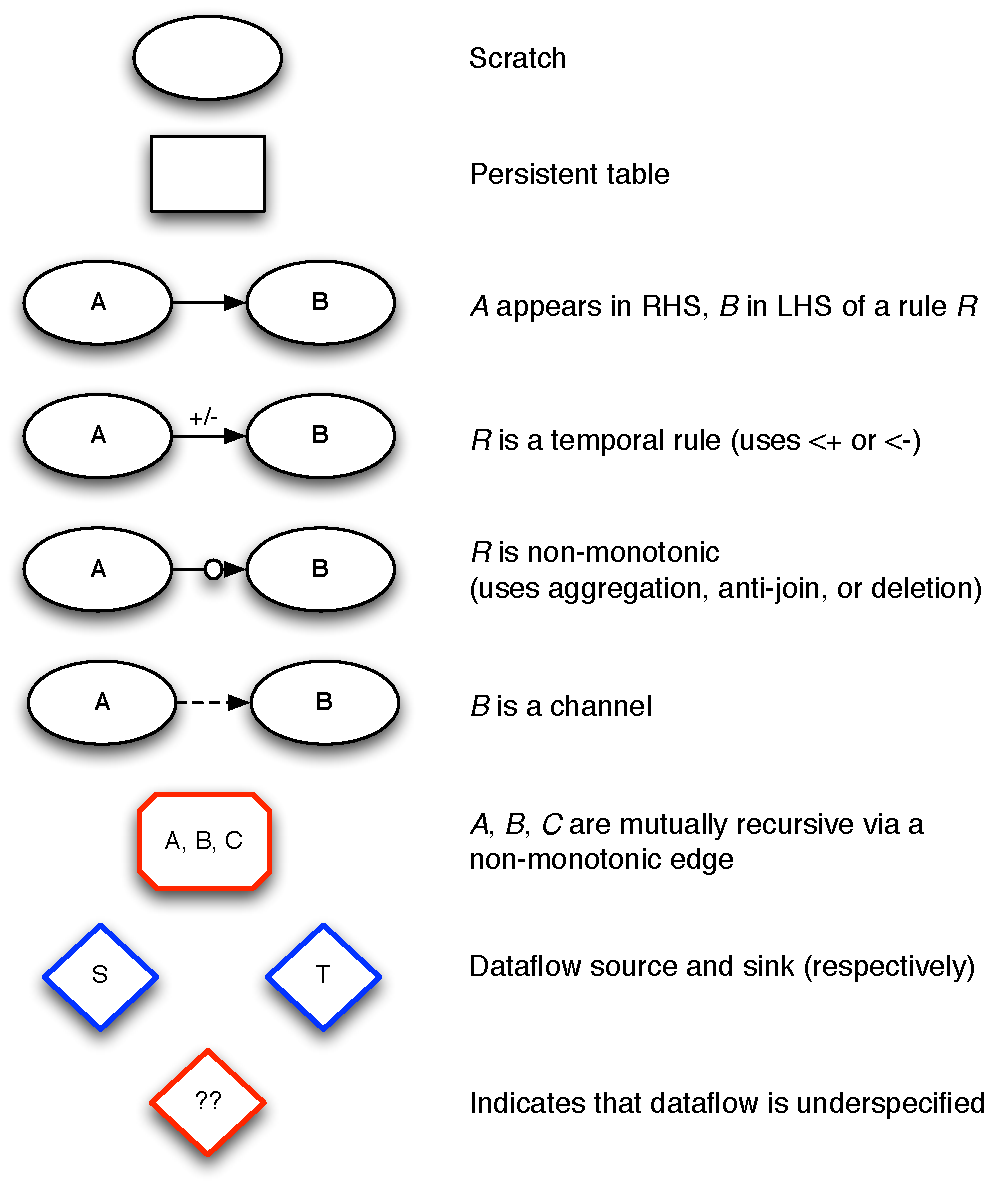
\includegraphics[width=1.1\linewidth]{fig/mittalk_legend.pdf}
\vspace{-10pt}
\caption{Visual analysis legend.}
\label{fig:analysis-legend}
\vspace{-2pt}
\end{figure}






\begin{figure}[t]
\begin{scriptsize}
\begin{lstlisting}
module KVSProtocol
  def state
    super
    interface input, :kvput, ['client', 'key', 'reqid'], ['value']
    interface input, :kvget, ['reqid'], ['key']
    interface output, :kvget_response, ['reqid'], ['key', 'value']
  end
end



\end{lstlisting}
\centering
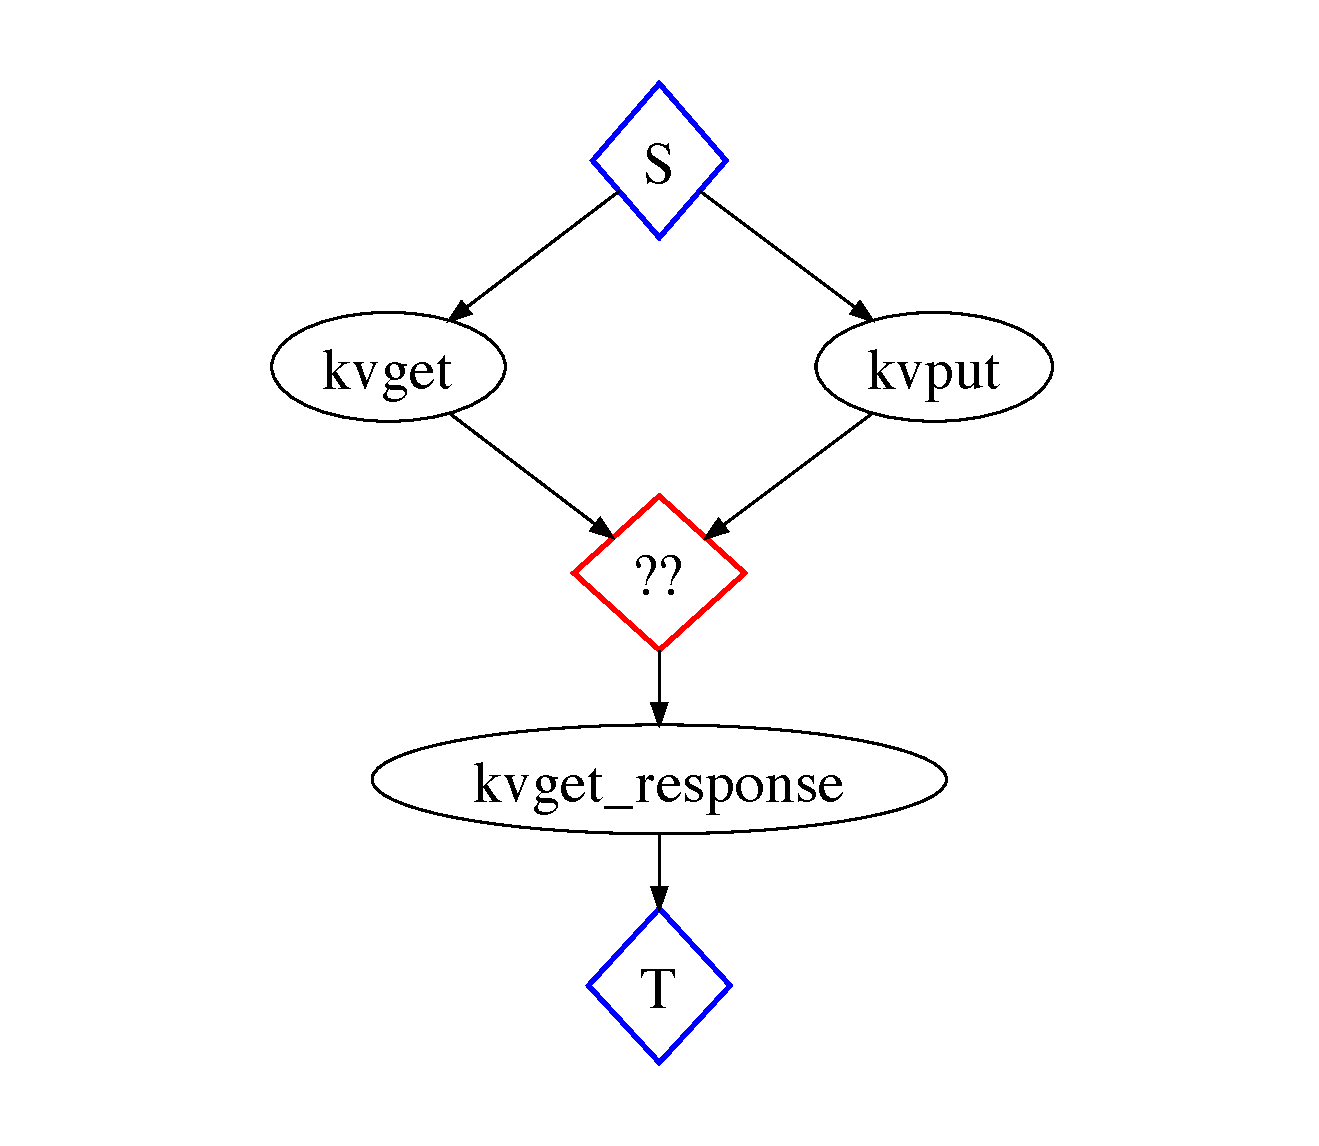
\includegraphics[width=0.4\linewidth]{fig/kvs_proto_pdg.pdf}
\vspace{-10pt}
\caption{Key/value store protocol.}
\label{fig:kvs-proto}
\end{scriptsize}
\vspace{-2pt}
\end{figure}


\begin{figure}[t]
\begin{scriptsize}
\begin{lstlisting}
module BasicKVS
  include KVSProtocol

  def state
    super
    table :bigtable, ['key'], ['value'] (*\label{line:kvs-state}*)
  end

  declare
  def mutate
    bigtable <+ kvput.map {|p| [p.key, p.value] } (*\label{line:kvs-put}*)
    jst = join [bigtable, kvput], [bigtable.key, kvput.key] (*\label{line:kvs-join}*)
    bigtable <- jst.map {|b, p| b } (*\label{line:kvs-clean}*)
  end

  declare
  def get
    getj = join [kvget, bigtable], [kvget.key, bigtable.key] (*\label{line:kvs-getjoin}*)
    kvget_response <= getj.map do |g, t|
      [g.reqid, t.key, t.value]
    end
  end
end


\end{lstlisting}
\centering
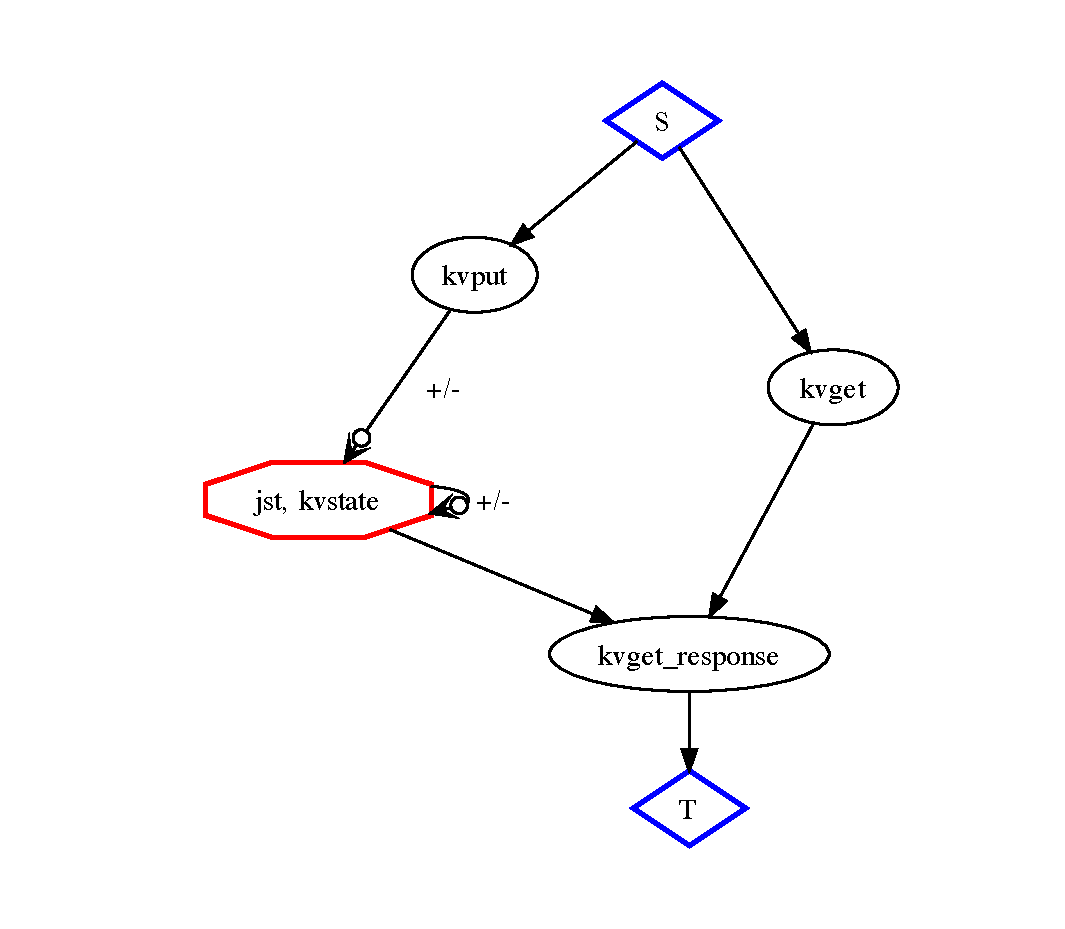
\includegraphics[width=0.55\linewidth]{fig/basickvs.pdf}
\vspace{-10pt}
\caption{Key/value store implementation.}
\label{fig:kvs-impl}
\end{scriptsize}
\vspace{-2pt}
\end{figure}


\begin{comment}
\begin{figure}[t]
\centering
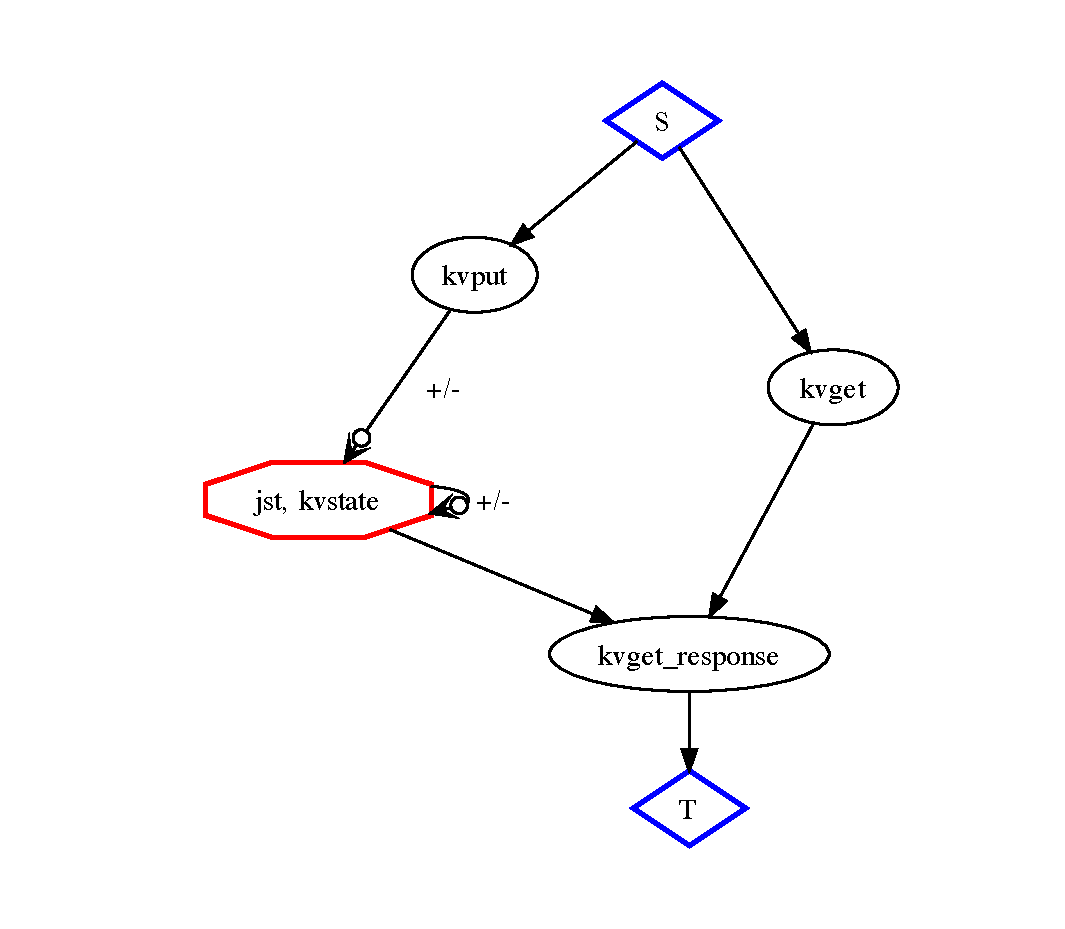
\includegraphics[width=0.5\linewidth]{fig/basickvs.pdf}
\vspace{-10pt}
\caption{Key/value store analysis.}
\label{fig:pdg-kvs-analysis}
\vspace{-2pt}
\end{figure}
\end{comment}

\begin{figure}[t]
\begin{scriptsize}
\begin{lstlisting}
module ReplicatedKVS
  include BasicKVS
  include MulticastProtocol

  def state
    interface input, :kvput, ['client', 'key', 'reqid'], ['value']  (*\label{line:rep-put}*)
  end

  declare
  def local_indir
    send_mcast <= kvput.map do |k| (*\label{line:send-mcast-beg}*)
      unless members.include? [k.client]  (*\label{line:not-rep}*)
        [k.reqid, [@addy, k.key, k.reqid, k.value]]   (*\label{line:marshall}*)            
      end
    end (*\label{line:send-mcast-end}*)
    
    kvput <= mcast_done.map {|m| m.payload }  (*\label{line:mcast-done}*)

    kvput <= pipe_chan.map do |d| (*\label{line:mcast-peer-beg}*)
      if d.payload.fetch(1) != @addy
        d.payload
      end
    end (*\label{line:mcast-peer-end}*)
  end
end

\end{lstlisting}
\vspace{-10pt}
\caption{Replicated key/value store.}
\label{fig:kvs-repl}
\end{scriptsize}
\vspace{-2pt}
\end{figure}
\section{Case Study}
\label{sec:case}

%%\wrm{Re-do case studies in Bud} \wrm{Break cart development down into
%%iterations} \wrm{How does the language naturally lead us to an order
%%independent style?  Talk about inserting all sorts of exotic stuff like queues
%%if we want a highly order-dependent imperative style.}

\begin{comment}

\jmh{We discussed the following on the phone.  (1) Handle shopping in two styles: destructive updates, and disorderly accumulation of increment/decrement.  (2) Do analysis on them to detect need for coordination in only the first, show that (annotated) 2PC removes the compiler warning.  (3) Deploy destructive+2PC on EC2 and show practical benefits of avoiding coordination.  (4) Evolve the program with new rules for checkout and/or inventory, show how the disorderly version is no longer monotonic.  Fix that  with 2PC where needed.  Also make sure the destructive version works with the new rules.  Now show that the disorderly version is still better than the destructive one, by coordinating only where needed.}

\jmh{Finally, show what would happen if you didn't coordinate the inventory bit, but tracked taint.  Note that tainted output is the stuff where programmers need to write compensation logic.}

\end{comment}

%%In this section, we implement two different styles of distributed shopping cart
%%applications in Bud.  First, we implement a ``destructive,'' overwriting
%%shopping cart application using a simple key-value store implemented in Bud.
%%Second, we implement a ``disorderly'' cart which accumulates updates in a 
%%set-wise fashion and describes how to combine the updates into a final result.

\jmh{Blah blah intro.}

We begin with a shopping
cart built on a key-value store abstraction.  Each cart is a pair \texttt{[key,value]}, where \texttt{key} is a unique 
session identifier, and \texttt{value} is a Ruby array
representing the set of items contained in the cart at any time.  Addition
and deletion actions to a cart result in ``destructive'' overwrites,
replacing the value associated with the key with a new array reflecting
the additions.  Deletion from an empty cart is ignored. 

Figure~\ref{fig:pdg-destructive} shows the Bloom code for this design.
The 
\textbf{scratch} \texttt{kvstore} is defined by the KeyValueStore module (XXX lines of Bloom not shown here), 
which the shopping cart extends via inheritance.
%; it is used in a manner analogous to the \emph{put} function for hash tables.  
The set of shopping carts, represented by the persistent \textbf{table} \texttt{bigtable}, is kept 
consistent across replicas by shipping \texttt{kvstore} tuples to other servers.
%%\jmh{Line numbers seem messed up.}

We begin describing the logic from the outside:
cart updates are transmitted from the client in line 28,
thereafter appearing in the \texttt{action\_msg} \textbf{channel} at a server replica.
\jmh{which server replica?  all server replicas??}
For each such arriving tuple,
line 2 probes the \texttt{bigtable} collection for a matching
session.  If none is found (i.e., the cart did not previously exist), lines 2-6 are evaluated, generating
the key with an appropriately initialized array. 
Otherwise the join conditions
in lines 10-11 will be met and lines 12-18 will instead be evaluated, ``replacing'' the value at the next timestep with an appropriately-modified new value.
Finally, when a checkout message is received, the value in \texttt{bigtable}
associated with the given session is extracted (via the join on lines 22-23)
and sent back to the client.

Figure~\ref{fig:} shows an alternative shopping cart implementation, in which
updates are accumulated in a disorderly fashion and summarized only at 
checkout.  Line 0 appends all client updates to the persistent table 
\texttt{cart\_action}.  Lines 2-3 define \texttt{action\_cnt} as an aggregate
over \texttt{cart\_action}, in the style of an SQL group-by statement: for
each item associated with a cart, we separately count the number of times it was added and the number of times it was deleted.
\jmh{what's up with lines 5-9?  initialize number of deletions to 0...to avoid failed join of additions with no deletions, right?  Maybe less confusing to do another rule for status that antijoins additions to deletions.  Or we could hack up an outerjoin syntax.}
\paa{I've frequently wanted an outerjoin syntax.  anti join? do you mean a 
'subquery' with unlesss..include? ?}
Lines 11-16 define the collection \texttt{status} as a 3-way
join between the \texttt{checkout} message and two copies of 
\texttt{action\_cnt} (one corresponding to additions and one to deletions),
and for each item, compute its final quantity in the cart as the difference of the two counts
in line 14.  A \texttt{response} message containing the quantity is then sent 
to the client in lines 18-22.  Because the disorderly implementation does not
use a separate storage system, it must replicate its own state to replicas 
via multicast (lines 24-26).


\begin{figure}[t]
\begin{scriptsize}
\begin{verbatim}

0: kvstore <= action_msg.map do |a|
1:   if not bigtable.map{|b| b.key}.include? a.session
2:     if a.action == "Add"
3:       [a.server, a.client, a.session, a.reqid, [a.item]]
4:     elsif a.action == "Del"
5:       [a.server, a.client, a.session, a.reqid, []]
6:     end
7:   end
8: end
9: 
10: kvstore <= join([bigtable, action_msg]).map do |b, a|
11:   if b.key == a.session
12:     if a.action == "Add"
13:       [a.server, a.client, a.session, a.reqid, b.value.push(a.item)]
14:     elsif a.action == "Del"
15:       copy = b.value.clone;
16:       copy.delete_at(copy.index(a.item));
17:       [a.server, a.client, a.session, a.reqid, copy]
18:     end
19:   end
20: end
21:
22: response_msg <+ join([bigtable, checkout_msg]).map do |s, c|
23:   if s.key == c.session
24:     [c.client, c.server, s.key, s.value]
25:   end
26: end
27: 
28: action_msg <+ client_action.map{|a| a}


\end{verbatim}
\end{scriptsize}
\caption{Destructive Cart Implementation}
\label{fig:pdg-destructive}
\end{figure}

\begin{figure}[t]
\centering
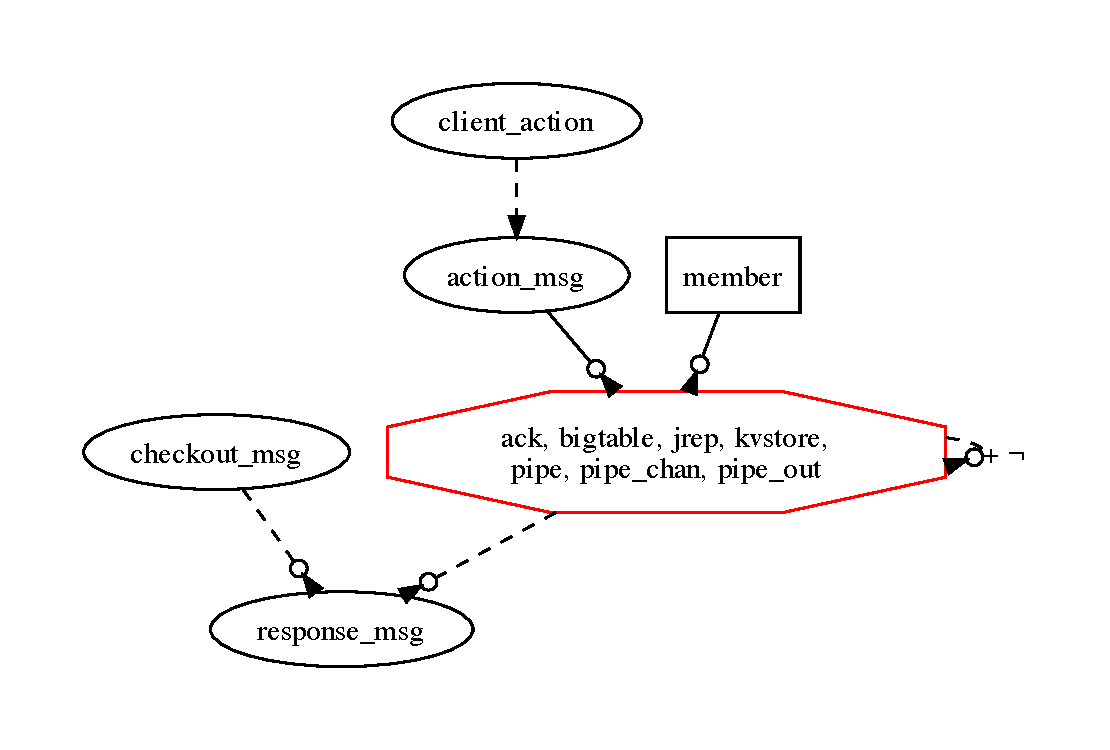
\includegraphics[width=0.9\linewidth]{fig/destructive.pdf}

\caption{Destructive Cart Analysis, with temporal cycles collapsed}
\label{fig:pdg-destructive-analysis}
\end{figure}


\subsection{Analysis}


For each cart, we apply whole-program analysis techniques to discover points of 
order.  The Bud interpreter automatically generates
a graphical representation of the dependency graph of collections through rules,
(and hence the 
flow of tuples) as a staged dataflow.  Each node in the graph is either
a collection or a cluster of collections (as described below).  A directed edge from node $A$ to node $B$ captures the fact that $B$ is in the lhs of a Bloom statement with $R$ in the rhs (or in a join expression in the rhs).  Edges are annotated based on the operators and lhs types in the rules.  Rules that involve synchronous timesteps---i.e. a \texttt{$<$+} operator with a {\bf table} lhs---are marked with a $+$.  Rules that involve asynchronous messaging---i.e., a \texttt{$<+$} operators with a {\bf channel lhs}---are indicated by a dashed line.  Nonmonotonic rhs predicates result in edges marked with a $\lnot$.  Strongly connected components having both a $\lnot$ and a $+$ edge are grouped into ``temporal clusters'', 
%%\jmh{capturing what? the fact that they must recurse over multiple timesteps?}
collapsing the mutually dependent collections into a single node.  All edges
incident to a temporal cluster, including the self-edge, are points of order,
as are any negated edges.
%%Individual monotonic components 
%%(or strata) are surrounded by a dotted rectangle.  A point of order occurs
%%wherever an edge crosses strata, or at any self-edge attached to a temporal cluster.
Points of order are indicated by lightning bolts.

To resolve a point of order, the programmer may add coordination logic, which typically ensures  ordered delivered tuples, and/or guarantees that a boundary condition has been irrevocably crossed (e.g., there will be no more tuples).
% Instead of reanalyzing the augmented program, we associate coordination code
% with an annotation that can
% be interpreted as a contract about a point of order.  Such contracts will
% typically guarantee an ordering over arriving tuples, or guarantee a 
% a barrier-passing condition (e.g., indicating that there will be no more tuples).

\jmh{the subsequent discussion should be pared down and made simple.  updates are non-monotonic.  we see it in the points of order.  If we resolve using coordination a la 2PC, we get a round of coord for every client action.  This is the kind of thing Amazon didn't like for availability.  However, if we examine the disorderly figure, we see that the point of order is at checkout only, which is what Amazon wanted.}
%%Intuitively, the ``destructive'' cart based on
%%array mutation should be non-monotonic due to the transience of its state; this should make it sensitive to the order
%%of its inputs.
Although there is no syntactically obvious non-monotonicity in the destructive
cart code as shown, the underlying key-value store uses the \texttt{$<$-} operator to model updateable state, which results in non-monotonicity.\footnote{Our full-length paper expands the SCC to analyze the
key-value store in detail.}
The global analysis shown in Figure~\ref{fig:pdf-destructive}
indicates that there are
points of order between \texttt{action\_msg} and the temporal cluster,
and between the temporal cluster and itself.
%%This means that the arrival 
%%timing and ordering of both client updates (via \texttt{iaction}) and
%%server replication (via the meta-edge in the temporal cycle from 
%%\texttt{kvstore} to itself) may affect the
%%end results.  
To ensure a consistent final state across all replicas, we may require coordination
between client and server at every update to the cart, and between the 
server and all replicas at each update.   

%%We can easily achieve coordination without modifying the cart implementation
%%by redefining the key-value store to extend
%%a reliable or quorum-based delivery module instead of the best-effort module
%%that the basic key-value store extends, and require acknowledgement from a server or a %%quorum of servers, respectively.
%%The simplest (and least performant) approach is to require unanimous quorum,
%%approximating ``eager replication''~\cite{dangers} via two-phase commit.
A programmer could resolve this point of order by adapting the key-value store
to require reliable delivery to all replicas before acknowledging a client update, by
making the key-value store inherit from a superclass providing a reliable delivery
abstraction (6 LOC).
Such ``eager replication''~\cite{dangers} would incur a cost of a round of messages
per server per client update, and substantially decrease system throughput.  
Because we only care about the set of elements contained in the value array
and not its order, we might be tempted to argue that 
the shopping cart application is eventually consistent
when asynchronously updated, and forego the synchronization.  Unfortunately, such informal reasoning can hide serious bugs: consider what happens if a delete update is received
before the addition it was intended to cancel.



\begin{figure}[t]
\begin{scriptsize}
\begin{verbatim}
0:  cart_action <= action_msg.map { |c| [c.session, c.item, c.action, c.reqid] }
1:
2:  action_cnt <= cart_action.group([cart_action.session, 
3:    cart_action.item, cart_action.action], count(cart_action.reqid))
4:
5:  action_cnt <= cart_action.map do |a| 
6:    unless cart_action.map{|c| [c.session, c.item] if c.action == "D"}.include? [a.session, a.item] 
7:      [a.session, a.item, 'D', 0]
8:    end 
9:  end
10: 
11: status <= join([action_cnt, action_cnt, checkout]).map do |a1, a2, c| 
12:   if a1.session == a2.session and a1.item == a2.item 
13:   and a1.session == c.session and a1.action == "A" and a2.action == "D"
14:     [a1.session, a1.item, a1.cnt - a2.cnt] if (a1.cnt - a2.cnt) > 0
15:   end
16: end
17:
18: response_msg <= join([status, checkout]).map do |s, c| 
19:   if s.session == c.session
20:     [c.client, c.server, s.session, s.item, s.cnt]
21:   end
22: end
23: 
24: action_msg <+ join([action_msg, member]).map do |a, m|
25:   [m.player, a.server, a.session, a.item, a.action, a.reqid]
26: end
27: 
28: checkout_msg <+ join([checkout_msg, member}).map do |c, m|
29:   [m.player, c.server, c.session, c.reqid]
30: end


\end{verbatim}
\end{scriptsize}
\caption{Disorderly Cart Implementation}
\label{fig:pdg-disorderly}
\end{figure}

\begin{figure}[t]
\centering
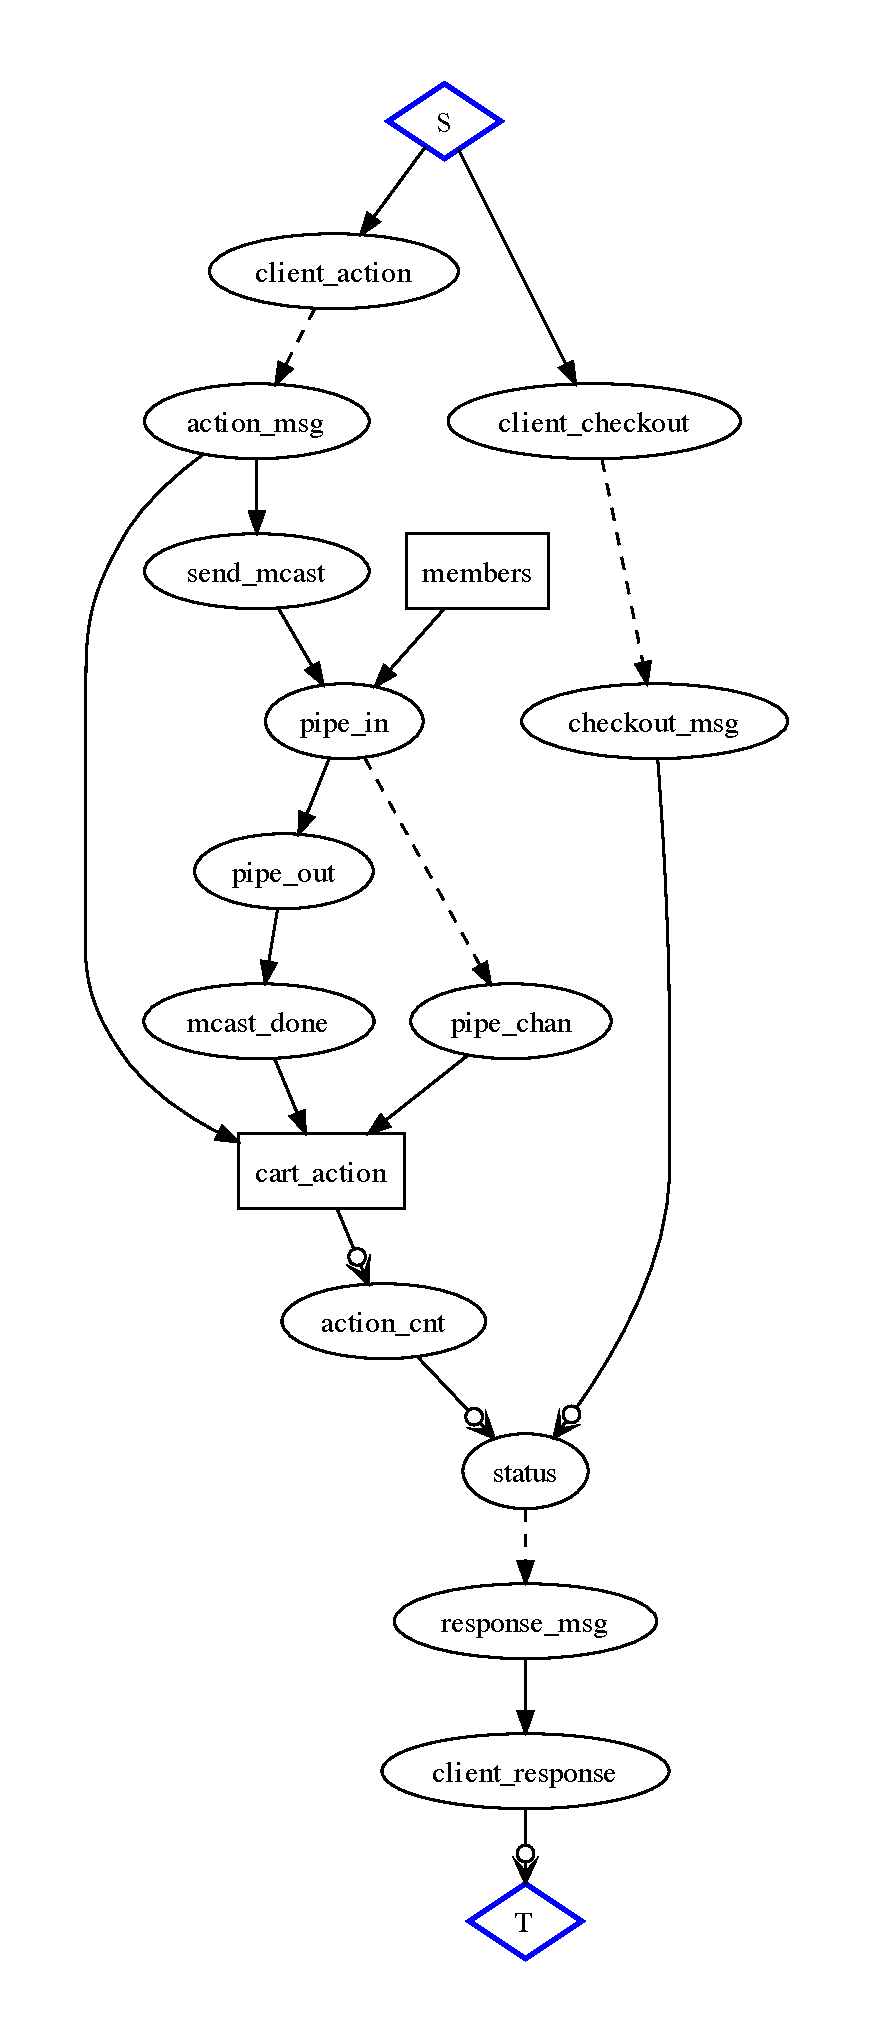
\includegraphics[width=0.7\linewidth]{fig/disorderly.pdf}
\caption{Disorderly Cart Analysis}
\label{fig:pdg-disorderly-analysis}
\end{figure}




Turning our attention to the disorderly figure,
\begin{comment}
 shows dotted lines indicating that 
\texttt{action\_msg} (owned by the server) is derived from \texttt{client\_action} 
(owned by the client) via an asynchronous message, and that \texttt{action\_msg} 
derives itself via messages when it is replicated.  However, the analysis
shows that because these derivations are strictly monotonic, no points of
order are crossed.  Hence, clients may send and servers may replicate 
updates without any coordination: regardless of timing and ordering, the end
result will be the same.

The analysis does indicate a point of order at checkout, when a \texttt{checkout}
message is joined with an aggregate over the set of updates.  While the 
accumulation of state has been monotonic, summarization of the cart state
requires us to assume (or prove) that there will be no further updates.
Consider a checkout message and a final update message racing from a client
to one of the replicas: the order in which they arrive will surely affect
the contents of the response message.  
\end{comment}
we see that communication (via \texttt{action\_msg}) between client and server
and between servers and replicas crosses no points of order, so all such
communication will converge to the same final state without coordination.
There is, however, a point of order at checkout, when a \texttt{checkout}
message is joined with an aggregate over the set of updates.  While the 
accumulation of state has been monotonic, summarization of the cart state
requires us to assume (or prove) that there will be no further updates.
Consider a checkout message and a final update message racing from a client
to one of the replicas: the order in which they arrive will surely affect
the contents of the response message.  
We need only coordinate once per session to
ensure that the response to the client is deterministic.

Like embarrassing parallelism in parallel computing, strictly monotonic programs
are rare in the distributed systems domain.  In this running example we studied
two candidate implementations of a simple distributed application with the aid of
our tool, and discovered that both have points of order.  Deciding that the disorderly
approach is ``better'' required us to apply domain knowledge: checkout happens
once per session, and is a more efficient coordination point than state update and replication, 
which occur repeatedly -- this is not unlike synchronizing on read rather than write 
in write-dominant systems generally.  Our analysis assisted us by highlighting the few locations where program correctness may depend upon costly synchronization, which may
result in decreased throughput and availability.  

\jmh{Challenge text that was kicking around and needs to be addressed here: we don't really say how we discourage a programmer from a destructive implementation, or help them migrate from that implementation to a better one.  Ideally we'd find ways to ``push back'' coordination requirements to local nodes and/or points of the program that don't have latency constraints.}


\section{Related Work}
\label{sec:relwork}
The shopping cart case study in Section~\ref{sec:case} was motivated by the
Amazon Dynamo paper~\cite{dynamo}, as well as the related discussion by Helland
and Campbell~\cite{quicksand}. Systems with loose consistency requirements have
been explored in depth by both the systems and database management communities
(e.g.,~\cite{sagas,leases,dangers,bayou}); we do not attempt to provide
an exhaustive survey here.

The Bloom language is inspired by earlier work that attempts to integrate
databases and programming languages.  This includes early research such as
Gem~\cite{gem} and more recent object-relational mapping layers like Ruby on
Rails.  Unlike these efforts, Bloom is targeted at the development of both
distributed infrastructure and distributed applications, so it does not make any
assumptions about the presence of a database system ``underneath it.''  Given
our prototype implementation in Ruby, it is tempting to integrate Bud with
Rails; we have left this for future work.

Our work on Bloom bears a resemblance to the Reactor
language~\cite{reactors}. Both languages target distributed programming and are
grounded in Datalog. Moreover, both languages combine declarative rules and
state into a single program construct. While Bloom uses a syntax inspired by
object-oriented languages, Reactor takes a more explicitly agent-oriented
approach. Reactor also includes synchronous coupling between agents as a
primitive; we have opted to only include asynchronous communication as a
language primitive and to provide synchronous coordination between nodes as a
library. Another significant different is that, like many rule-based languages,
Reactor includes some imperative constructs (e.g., \ldots), whereas rules in
Bloom are purely declarative.

Another recent language related to our work is Coherence~\cite{coherence}, which
also embraces ``disorderly'' programming. Unlike Bloom, Coherence is not
designed for distributed computing and is not based on logic programming.

There is a long history of attempts to design programming languages more
suitable to parallel and distributed systems; for example, Argus~\cite{argus}
and Linda~\cite{linda}.  Again, we do not hope to survey that literature here.
More pragmatically, Erlang is an oft-cited choice for distributed programming in
recent years.  Erlang's features and design style encourage the use of
asynchronous lightweight ``actors.''  As mentioned previously, we did a simple
Bloom prototype DSL in Erlang (which we cannot help but call ``Bloomerlang''),
and there is a natural correspondence between Bloom-style distributed rules and
Erlang actors.  However there is no requirement for Erlang programs to be
written in the disorderly style of Bloom. It is not obvious that typical Erlang
programs are significantly more amenable to a useful points-of-order analysis
than programs written in any other functional language.  For example, ordered
lists are basic constructs in functional languages, and without program
annotation or deeper analysis than we need to do in Bloom, any code that
modifies lists would need be marked as a point of order, much like our
destructive shopping cart.  We believe that Bloom's ``disorderly by default''
style encourages more disorderly programming; we know that its roots in database
theory bore fruit in terms of our analysis.  While we would be happy to see the
analysis ``ported'' to currently popular distributed programming environments,
it may be that design patterns using Bloom-esque disorderly programming are the
natural way to achieve this.

\section{Conclusion}
\label{sec:conclusion}
And thus, we conclude.
\section{Acknowledgments}
Ras Bod\'{\i}k and Tyson Condie were intimately involved in discussions
surrounding the development of \lang.  We are also indebted to Mark Utting and
Erik Meijer for conversation and inspiration from their Starlog and LINQ
experiences respectively, and to Phil Bernstein for suggestions on future work.
Thanks to Jesse Trutna and Kuang Chen for comments on the paper. This work was
supported by NSF grants 0803690, 0722077 and 0713661, Air Force Office of
Scientific Research award 22178970-41070-F, the Natural Sciences and
Engineering Research Council of Canada, and gifts from Yahoo Research, IBM
Research and Microsoft Research.


\bibliographystyle{abbrv}
\bibliography{cidr11,declarativity}

\end{document}
